\documentclass[12pt]{article}
\usepackage{../light}
%\newcommand{\Var}{\mathop{\textup{Var}}\nolimits}
\newcommand{\var}[1]{\Var\left[#1\right]}

\hidesolutions
%\showsolutions

\begin{document}

\newcommand{\prsub}[2]{\mathop{\textup{Pr}_{#1}}\nolimits\left(#2\right)}

\recitation{24}{December 5, 2008}

%%%%%%%%%%%%%%%%%%%%%%%%%%%%%%%%%%%%%%%%%%%%%%%%%%%%%%%%%%%%%%%%%%%%%%%%%%%%%%%

\begin{theorem}
\label{th:num-events}
Let $E_1, \ldots, E_n$ be events, and let $X$ be the number of these
events that occur. Then:
%
\[
\ex{X} = \pr{E_1} + \pr{E_2} + \ldots + \pr{E_n}
\]
\end{theorem}

\begin{theorem}[Markov's Inequality]
\label{th:markov}
Let $X$ be a nonnegative random variable.  If $c > 0$, then:
%
\[
\pr{X \geq c} \leq \frac{\ex{X}}{c}
\]
\end{theorem}

\begin{theorem}[Chebyshev's Inequality]
\label{th:chebyshev}
For all $x > 0$ and any random variable $R$,
$$\pr{|R-\ex{R}| \geq x} \leq \frac{\var{R}}{x^2}$$
\end{theorem}

\begin{theorem}[Union Bound]
\label{th:union}
For events $E_1, \ldots, E_n$:
%
\[
\pr{E_1 \cup \ldots \cup E_n} \leq \pr{E_1} + \ldots + \pr{E_n}
\]
\end{theorem}

\begin{theorem}[``Murphy's Law'']
\label{th:murphy}
If events $E_1, \ldots E_n$ are mutually independent and $X$ is the
number of these events that occur, then:
%
\[
\pr{E_1 \cup \ldots \cup E_n} \geq 1 - e^{-\ex{X}}
\]
\end{theorem}

\begin{theorem}[Chernoff Bounds]
\label{th:chernoff}
Let $E_1, \ldots, E_n$ be a collection of mutually independent events,
and let $X$ be the number of these events that occur.  Then:
%
\begin{align*}
\pr{X \geq c \ex{X}} & \leq e^{\textstyle -(c \ln c - c + 1) \ex{X}}
    & \text{when $c > 1$}
\end{align*}
\end{theorem}

%\begin{corollary}
%\label{cor:chernoff}
%The second and third bounds in Theorem~\ref{th:chernoff} remain valid
%when all instances of $\ex{X}$ are replaced by an upper bound on the
%expectation of $X$.
%\end{corollary}

%%%%%%%%%%%%%%%%%%%%%%%%%%%%%%%%%%%%%%%%%%%%%%%%%%%%%%%%%%%%%%%%%%%%%%%%%%%%%%%

\newpage

\section{Getting Dressed}
Sometimes I forget a few items when I leave the house in the morning.

 For example, here are probabilities that I forget various
pieces of footwear:
%
\[
\begin{array}{p{2in}l}
left sock & 0.2 \\
right sock & 0.1 \\
left shoe & 0.1 \\
right shoe & 0.3
\end{array}
\]
%
\begin{itemize}
\item[a.]

Let $X$ be the number of these that I forget.  What is $\ex{X}$?

\solution[\vspace{1in}]{By Theorem~\ref{th:num-events}, the expected
number of events that happen is the sum of the event probabilities.
So,
%
\[
\ex{X} = 0.2 + 0.1 + 0.1 + 0.3 = 0.7
\]
}

\item[b.] Upper bound the probability that I forget one or more items.
Make no independence assumptions.

\solution[\vspace{1in}]{By the Union Bound, the probability that I
forget something is at most:
%
\[
0.1 + 0.1 + 0.2 + 0.3 = 0.7
\]
}

\item[c.] Use the Markov Inequality to upper bound the probability that I
forget 3 or more items.

\solution[\vspace{1.5in}]{
\begin{align*}
\pr{X \geq 3} \leq \frac{\ex{X}}{3} = \frac{7}{30}
\end{align*}
}

\item[d.] Now suppose that I forget each item of footwear independently. Use Chebyshev's Inequality to upper bound the probability that I forget two or more items.

\solution[\vspace{1.5in}]{ Let $X_1$ be the event I bring my left sock, $X_2$ my right sock, $X_3$ my left shoe, and $X_4$ my right shoe. Then $\ex{X_1} = .2$, $\ex{X_2} = .1$, $\ex{X_3} = .1$, and $\ex{X_4} = .3$. Moreover, since the $X_i$ are Bernoulli random variables (binomial with $n=1$), we have $\var{X_1} = .2(1-.2) = .16, \var{X_2} = .1(1-.1) = .09, \var{X_3} = .1(1-.1) = .09$, and $\var{X_4} = .3(1-.3) = .21$.
\\\\
Let $X = \sum_{i=1}^4 X_i$. Then $\ex{X} = \sum_{i=1}^4 \ex{X_i} = .2 + .1 + .1 + .3 = .7$. Since the $X_i$ are independent, $\var{X} = \sum_{i=1}^4 \var{X_i} = .16 + .09 + .09 + .21 = .55$. Now by Chebyshev's Inequality,
\begin{align*}
\pr{X \geq 2}
    & \leq \pr{|X-.7| \geq 1.3}\\
    & = \pr{|X-\ex{X}| \geq 1.3}\\
    & \leq \frac{\var{X}}{1.3^2}\\
    & = \frac{.55}{1.3^2}\\
    & \leq .326
\end{align*}
}

\item[e.] Use Theorem~\ref{th:murphy} to lower bound the probability that I forget
one or more items.

\solution[\vspace{1.5in}]{Plugging into Theorem~\ref{th:murphy}, the
probability that I forget one or more items:
%
\[
1 - e^{-\ex{X}} = 1 - e^{-0.7} = 0.503\ldots
\]
}

\iffalse
\item[f.] I'm supposed to remember many other items, of course: clothing,
watch, backpack, notebook, pencil, kleenex, ID, keys, etc.  Let $X$ be
the total number of items I remember.  Suppose I remember items
mutually independently and $\ex{X} = 36$.

Give an upper bound on the probability that I remember 18 or fewer
items.

\solution[\vspace{2in}]{
By the first Chernoff inequality:
%
\begin{align*}
\pr{X \leq 18}
    & = \pr{X \leq (1 - 1/2) \ex{X}} \\
    & \leq e^{-(1/2)^2 36 / 2} \\
    & = e^{-9/2}
\end{align*}
}
\fi

\item[g.] 
I'm supposed to remember many other items, of course: clothing,
watch, backpack, notebook, pencil, kleenex, ID, keys, etc.  Let $X$ be
the total number of items I remember.  Suppose I remember items
mutually independently and $\ex{X} = 36$.
Use Chernoff's Bound to give an upper bound on the probability that I remember 48 or
more items.

\solution[\vspace{2in}]{
By the Chernoff Bound,
%
\begin{align*}
\pr{X \geq 48}
    & = \pr{X \geq (1 + 1/3) \ex{X}} \\
    & \leq e^{-(4/3 \ln 4/3 - 4/3 + 1) \cdot 36} \\
    & \approx .1638\\
\end{align*}
}

\item[h.] Give an upper bound on the probability that I remember $108$ or
more items.

\solution{By the Chernoff Bound,
%
\begin{align*}
\pr{X \geq 108}
    & = \pr{X \geq 3 \cdot \ex{X}} \\
    & \leq e^{-(3 \ln 3 - 3 + 1) \cdot 36} \\
    & \leq e^{-46} \approx 1.05\times 10^{-20}.
\end{align*}
}

\end{itemize}

%%%%%%%%%%%%%%%%%%%%%%%%%%%%%%%%%%%%%%%%%%%%%%%%%%%%%%%%%%%%%%%%%%%%%%%%%%%%%%%

\newpage

\section{NxN Array}
A routing network called an \textit{$n \times n$ array} is shown below
for $n = 4$.  There is an input terminal and an output terminal
attached to every node.  But for clarity only one such pair of
terminals is shown.
%
\begin{center}
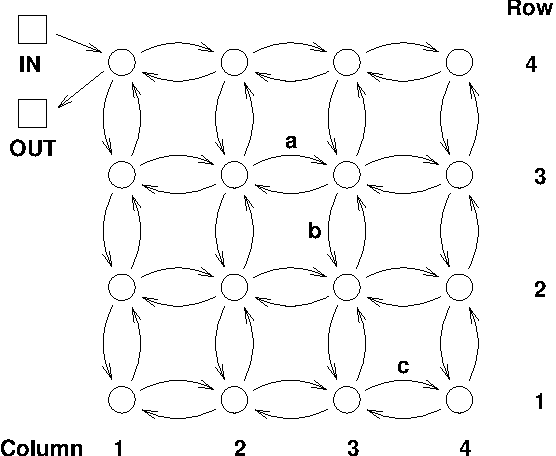
\includegraphics{2darray}
\end{center}
%
A packet travels between two nodes by first moving horizontally to the
correct column and then vertically to the correct row.  Suppose that
each input sends one packet to an output selected uniformly and
independently at random.  (So zero, one, two, or more packets can be
sent to a single output.)  The goal of this problem is analyze
congestion in an array using probability tools.

\begin{itemize}

\item[a.] What is the expected number of packets that cross edge $a$ in
the $4 \times 4$ array shown above?  Also, compute the expected number
of packets that cross edges $b$ and $c$.

\solution[\newpage]{Edge $a$ can only be crossed by packets
originating at the two nodes directly to its left.  Each of these
packets crosses edge $a$ if and only if its destination is in the
right half of the network, which happens with probability $1/2$.
Therefore, the expected number of packets crossing edge $a$ is $2
\cdot (1/2) = 1$.

Edge $b$ can be crossed by a packet originating at any of the 8 nodes
in the upper half of the network.  Each of these packets crosses edge
$b$ if and only if its destination is one of the two nodes directly
below $b$, which happens with probability $2/16 = 1/8$.  Thus, the
expected number of packets crossing edge $b$ is $8 \cdot (1/8) = 1$.

Edge $c$ can be crossed only by a packet originating at one of the
three nodes to its left.  Each of these packets crosses edge $c$ if
and only if its destination is in the righthand column, which happens
with probability $1/4$.  Therefore, the expected number of packets
that cross edge $c$ is $3 \cdot (1/4) = 3/4$.}

\item[b.] Now consider an $n \times n$ array.  Number the rows from 1 to
$n$ and number the columns from 1 to $n$.  What is the expected number
of packets that cross an upward edge $e$ from row $k$ to row $k+1$?

\solution[\vspace{2in}]{A packet crosses edge $e$ if and only if it
originates in one of the bottom $k$ rows and is destined for one of
the $n - k$ nodes directly above edge $e$.  Therefore, the expected
number of packets crossing edge $e$ is:
%
\[
nk \cdot \frac{n - k}{n^2} = \frac{k(n-k)}{n}
\]
}

\item[c.] What is the expected number of packets that cross a rightward
edge $f$ from column $k$ to column $k+1$?

\solution[\vspace{2in}]{A packet crosses edge $f$ if and only if it
originates at one of the $k$ nodes directly left of $f$ and is
destined for one of the $n-k$ rows to the right of $f$.  Thus, the
expected number of packets that cross edge $f$ is:
%
\[
k \cdot \frac{(n-k)n}{n^2} = \frac{k(n-k)}{n}
\]
}

\item[d.] Let $\mu$ be the expected number of packets crossing one of the
edges with the greatest expected congestion.  What is $\mu$?  (Assume
$n$ is even.)

\solution[\newpage]{The expressions from the two preceding problem
parts are both maximized when $k = n/2$.  Thus, for any edge joining
two different quadrants of the $n \times n$ array, the expected number
of crossing packets is $n / 4$.  So $\mu = n / 4$.}

\item[e.] Let $X$ be the number of packets that cross a particular edge.
We know that $\ex{X} \leq \mu$.  But if we're unlucky and something
weird happens, then $X$ might be much greater, which means that the
edge is especially congested.  Give an upper bound on:
%
\[
\pr{X \geq \mu + \sqrt{2 n \ln n}}
\]
%
Assume that $n$ is large enough that the second Chernoff inequality
applies.  (Note that $\sqrt{2 n \ln n}$ is quite small compared to
$\mu$ for large $n$; so we're trying to show that even small
deviations above the average congestion are unlikely.)

\solution[\vspace{3in}]{First, we need to rewrite the probability
above in a form suitable for a Chernoff bound argument:
%
\[
\pr{X \geq \frac{n}{4} + \sqrt{2 n \ln n}} = \pr{X \geq \frac{n}{4} (1 + \delta)}
\]
%
Here $\delta = \sqrt{32 \ln n / n}$.  Now we can apply the second
Chernoff inequality for sufficiently large $n$:
%
\begin{align*}
\pr{X \geq \frac{n}{4} (1 + \delta)}
    & \leq e^{-\delta^2 \ex{X} / 3} \\
    & = n^{-8/3}
\end{align*}
}

\item[f.] We've now shown that \textit{one} particular edge is not likely
to be congested.  However, an $n \times n$ array contains a
\textit{lot} of edges.  So there are a lot of different places where
something could go wrong.  Compute the number of edges in an $n \times
n$ array and then use the Union Bound to upper bound the probability
that $\mu + \sqrt{2 n \ln n}$ or more packets cross some edge.

\solution{The total number of edges is $4 (n - 1) n$.  Thus, by the
Union Bound, the probability that \textit{some} edge is crossed by
more than $\mu + \sqrt{2 n \ln }$ packets is at most:
%
\[
\frac{4 (n-1) n}{n^{8/3}} \leq \frac{4}{n^{2/3}}
\]

To illustrate the significance of these formulas, let's consider a huge
network with $n=10,000$.  In this case, the largest number of packets
expected at any edge is $2,500$.  By implementing edges with packet
capacity $2500 + \sqrt{2 \cdot 10000 \ln 10000} = 2930$, we will have a
network whose probability of overload failure is at most $4/(10000^{2/3})
< 0.01$.  That is, by implementing edges that can handle a load up to only
16\% higher than expected, the overall probability of overload failure
anywhere in the 400 million edge network is less than 1\%.}

\end{itemize}

%%%%%%%%%%%%%%%%%%%%%%%%%%%%%%%%%%%%%%%%%%%%%%%%%%%%%%%%%%%%%%%%%%%%%%%%%%%%%%%

\end{document}
